%%%%%%%%%%%%%%%%%%%%%% LLAMADAS AL SISTEMA - EJERCICIO 3 %%%%%%%%%%%%%%%%%%%%%%
\section{Ejercicio 3}
\subsection{Enunciado}
\begin{ejer}
    \textbf{3.[exit()\&wait()]} Modifica las llamadas \texttt{exit()} y \texttt{wait()} para que sigan la signatura de las
    funciones de \texttt{POSIX}, es decir: \texttt{int wait(int* status)} y \texttt{void exit(int status)}.
\end{ejer}
\subsection{Desarrollo}

\subsubsection{shell}
\begin{listing}[style=consola]
alumno@alumno xv6 % sed -i e 's/\bexit()/exit(0)g' @(!(sysproc.c|trap.c)|(*.c))
alumno@alumno xv6 % sed -i e 's/\bwait()/wait(0)g' @(!(sysproc.c|trap.c)|(*.c))
\end{listing}
\par Para que el sistema siga funcionando, hay que cambiar las llamadas a \texttt{exit} 
y \texttt{wait} que hay a lo largo del sistema operativo para que acepten un parámetro.

\subsubsection{xv6/user.h}
\begin{listing}
@@ -1,6 +1,10 @@
+   #define WIFEXITED(status)   (((status) & 0x7f) == 0)
+   #define WEXITSTATUS(status) (((status) & 0xff00) >> 8)
+   #define WIFSIGNALED(status) (((status) & 0x7f) != 0)
+   #define WEXITTRAP(status)   (((status) & 0x7f)-1)
    struct stat;
    struct rtcdate;
// system calls
    extern int fork(void);
-   extern int exit(void) __attribute__((noreturn));
+   extern int exit(int) __attribute__((noreturn));
-   extern int wait(void);
+   extern int wait(int*);
\end{listing}
\par Añadimos las macros definidas en \texttt{POSIX} y las funciones 
de llamada al sistema ahora aceptan los argumentos.

\subsubsection{xv6/defs.h}
\begin{listing}
@@ -104,4 +104,4 @@
//PAGEBREAK: 16
// proc.c
    int             cpuid(void);
-   void            exit(void);
+   void            exit(int);
@@ -119,3 +119,3 @@
    void            userinit(void);
-   int             wait(void);
+   int             wait(int*);
    void            wakeup(void*);
\end{listing}
\par Ajustamos las deficiones de las funciones \texttt{wait()} y \texttt{exit()}
para que puedan ser visibles ahora con los argumentos correctos para el código del sistema operativo.

\subsubsection{xv6/sysproc.c}
\begin{listing}
@@ -16,14 +16,17 @@
    int
    sys_exit(void)
    {
+       int exit_status;
+       if(argint(0, &exit_status) < 0)
+           return -1;
-       exit();
+       exit(exit_status);
        return 0;  // not reached
    }
    int
    sys_wait(void)
    {
        int *exit_status;
        if(argptr(0, (void**)&exit_status, sizeof(exit_status)) < 0)
            return -1;
-       return wait();
+       return wait(exit_status);
    }
\end{listing}
\par Adaptamos las funciones de implementación de las llamadas dentro del núcleo, \\
\texttt{sys\_exit()} y \texttt{sys\_wait()} para que acepten un entero (el estado 
de salida del proceso) y un puntero a enteros.

\subsubsection{xv6/proc.h}
\begin{listing}
@@ -48,5 +48,6 @@ struct proc {
        int killed;                  // If non-zero, have been killed
        struct file *ofile[NOFILE];  // Open files
        struct inode *cwd;           // Current directory
        char name[16];               // Process name (debugging)
+       int exit_status;             // Estatus de salida
    };
\end{listing}
\par Para poder guardar el código de salida del proceso tuvimos que añadir otro campo a la estructura \texttt{struct proc}.

\subsubsection{xv6/proc.c}
\begin{listing}
@@ -227,5 +227,5 @@ exit(int exit_satus)
    void
-   exit()
+   exit(int exit_status)
    {
        struct proc *curproc = myproc();
        struct proc *p;
@@ -241,3 +241,9 @@ exit(int exit_satus)
+       // TRAP
+       if (curproc->killed)
+            curproc->exit_status = exit_status+1;
+       else { // salida normal
+            curproc->exit_status = exit_status << 8;
+       }
        begin_op();
        iput(curproc->cwd);
        end_op();
@@ -276,3 +281,3 @@ wait(int *exit_status)
    int
-   wait()
+   wait(int *exit_status)
    {
@@ -292,3 +297,4 @@ wait(int *exit_status)
        pid = p->pid;
+       *exit_status = p->exit_status;
        kfree(p->kstack);
        p->kstack = 0;
@@ -303,6 +307,7 @@ wait(int *exit_status)
        p->name[0] = 0;
        p->killed = 0;
        p->state = UNUSED;
+       p->exit_status = 0;
        release(&ptable.lock);
        return pid;
    }
\end{listing}

\par En ambas funciones, hemos cambiado la definición para que admita el parámetro correspondiente.

\par En el caso del \texttt{exit()}, la funcionalidad es similar a la inical,
pero hemos añadido la implementación necesaria para que guarde en la estructura
del proceso el status correspondiente.

 %%% IMAGEN DE MACROS %%%
\begin{figure}[H]
	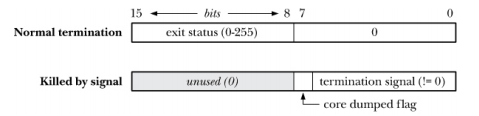
\includegraphics[width=\textwidth]{macroStatus}
	\centering
	\caption{Valor status devuelto por \texttt{wait()}.}
    	\label{fig:macroStatus}
\end{figure}

\par El status es calculado según las macros \texttt{WEXITSTATUS(status)} y
\texttt{WEXITTRAP(status)}, como indica la figura \ref{fig:macroStatus}. Estas están
definidas en el fichero \texttt{xv6/user.h} anteriormente citado.

\par La macro \texttt{WEXITSTATUS(status)} se queda con los 8 bits más significativos y
es usada por las terminaciones de programa normales.

\par Por otro lado, la macro \texttt{WEXITTRAP(status)}, se queda con los 7 bits menos
significativos y es usada por las terminaciones de programa debido a interrupciones. 

\par Para implementar el código de \texttt{exit()}, tenemos que pensar a la inversa y
colocar en los 8 bits más significatos o o 7 bits menos significativos según el caso
que corresponda.

\par En el caso del \texttt{wait()} lo que hace es colocar en
el parámetro que nos han pasado, que es un puntero, el valor del status entregado por el hijo, que estará almacenado en la estructura
del proceso del hijo.

\subsubsection{xv6/sh.c}
\begin{listing}
@@ -167,7 +167,12 @@ main(void)
        }
        if(fork1() == 0)
        runcmd(parsecmd(buf));
-       wait(0);
+       int exit_status;
+       wait(&exit_status);
+       if (WIFEXITED (exit_status))
+           printf (1, "Output code: %d\n", WEXITSTATUS (exit_status));
+       else if (WIFSIGNALED(exit_status))
+           printf (1, "Output code: %d\n", WEXITTRAP (exit_status));
    }
    exit(0);
}
\end{listing}
\par Modificamos la llamada al sistema \texttt{wait()} para que cada vez que 
ejecute un programa produzca el código de salida correspondiente.

\subsubsection{xv6/trap.c}
\begin{listing}
@@ -38,10 +38,10 @@ trap(struct trapframe *tf)
    {
    if(tf->trapno == T_SYSCALL){
        if(myproc()->killed)
-           exit();
+           exit(tf->trapno);
        myproc()->tf = tf;
        syscall();
        if(myproc()->killed)
-           exit();
+           exit(tf->trapno);
        return;
    }
@@ -100,2 +100,2 @@ trap(struct trapframe *tf)
        if(myproc() && myproc()->killed && (tf->cs&3) == DPL_USER)
-           exit();
+           exit(tf->trapno);
@@ -110,2 +110,2 @@ trap(struct trapframe *tf)
        if(myproc() && myproc()->killed && (tf->cs&3) == DPL_USER)
-           exit();
+           exit(tf->trapno);
\end{listing}

\par Modificamos el \texttt{xv6/trap.c} para enviarle a estos \texttt{exit()} el número de trap
como status de salida.

\subsection{Fichero de prueba}
\subsubsection{xv6/Makefile}
\begin{listing}
@@ -185,5 +185,6 @@ UPROGS=\
    _wc\
    _zombie\
    _date\
    _clear\
    _dup2test\
+   _exitwait\
\end{listing}
\par Para que nuestro programa esté disponible en el shell de \texttt{xv6}, insertamos 
\texttt{\_exitwait} a la definición \texttt{UPROGS} en el \texttt{Makefile}.

\subsubsection{Salida del fichero prueba}
\begin{listing}[style=consola]
    $ exitwait
    exit/wait with status test
    pid 6 exitwait: trap 0 err 0 on cpu 0 eip 0x52 addr 0xcfa4--kill proc
    pid 7 exitwait: trap 0 err 0 on cpu 0 eip 0x52 addr 0xcfa4--kill proc
    pid 8 exitwait: trap 0 err 0 on cpu 0 eip 0x52 addr 0xcfa4--kill proc
    pid 9 exitwait: trap 0 err 0 on cpu 0 eip 0x52 addr 0xcfa4--kill proc
    pid 10 exitwait: trap 0 err 0 on cpu 0 eip 0x52 addr 0xcfa4--kill proc
    pid 11 exitwait: trap 0 err 0 on cpu 0 eip 0x52 addr 0xcfa4--kill proc
    pid 12 exitwait: trap 0 err 0 on cpu 0 eip 0x52 addr 0xcfa4--kill proc
    pid 13 exitwait: trap 0 err 0 on cpu 0 eip 0x52 addr 0xcfa4--kill proc
    pid 14 exitwait: trap 0 err 0 on cpu 0 eip 0x52 addr 0xcfa4--kill proc
    pid 15 exitwait: trap 0 err 0 on cpu 0 eip 0x52 addr 0xcfa4--kill proc
    pid 16 exitwait: trap 0 err 0 on cpu 0 eip 0x52 addr 0xcfa4--kill proc
    pid 17 exitwait: trap 0 err 0 on cpu 0 eip 0x52 addr 0xcfa4--kill proc
    pid 18 exitwait: trap 0 err 0 on cpu 0 eip 0x52 addr 0xcfa4--kill proc
    pid 19 exitwait: trap 0 err 0 on cpu 0 eip 0x52 addr 0xcfa4--kill proc
    pid 20 exitwait: trap 0 err 0 on cpu 0 eip 0x52 addr 0xcfa4--kill proc
    pid 21 exitwait: trap 0 err 0 on cpu 0 eip 0x52 addr 0xcfa4--kill proc
    pid 22 exitwait: trap 0 err 0 on cpu 0 eip 0x52 addr 0xcfa4--kill proc
    pid 23 exitwait: trap 0 err 0 on cpu 0 eip 0x52 addr 0xcfa4--kill proc
    pid 24 exitwait: trap 0 err 0 on cpu 0 eip 0x52 addr 0xcfa4--kill proc
    pid 25 exitwait: trap 0 err 0 on cpu 0 eip 0x52 addr 0xcfa4--kill proc
    pid 26 exitwait: trap 0 err 0 on cpu 0 eip 0x52 addr 0xcfa4--kill proc
    pid 27 exitwait: trap 0 err 0 on cpu 0 eip 0x52 addr 0xcfa4--kill proc
    pid 28 exitwait: trap 0 err 0 on cpu 0 eip 0x52 addr 0xcfa4--kill proc
    pid 29 exitwait: trap 0 err 0 on cpu 0 eip 0x52 addr 0xcfa4--kill proc
    pid 30 exitwait: trap 0 err 0 on cpu 0 eip 0x52 addr 0xcfa4--kill proc
    pid 31 exitwait: trap 0 err 0 on cpu 0 eip 0x52 addr 0xcfa4--kill proc
    pid 32 exitwait: trap 0 err 0 on cpu 0 eip 0x52 addr 0xcfa4--kill proc
    pid 33 exitwait: trap 0 err 0 on cpu 0 eip 0x52 addr 0xcfa4--kill proc
    pid 34 exitwait: trap 0 err 0 on cpu 0 eip 0x52 addr 0xcfa4--kill proc
    pid 35 exitwait: trap 0 err 0 on cpu 0 eip 0x52 addr 0xcfa4--kill proc
    pid 36 exitwait: trap 0 err 0 on cpu 0 eip 0x52 addr 0xcfa4--kill proc
    pid 37 exitwait: trap 0 err 0 on cpu 0 eip 0x52 addr 0xcfa4--kill proc
    pid 38 exitwait: trap 0 err 0 on cpu 0 eip 0x52 addr 0xcfa4--kill proc
    pid 39 exitwait: trap 0 err 0 on cpu 0 eip 0x52 addr 0xcfa4--kill proc
    pid 40 exitwait: trap 0 err 0 on cpu 0 eip 0x52 addr 0xcfa4--kill proc
    pid 41 exitwait: trap 0 err 0 on cpu 0 eip 0x52 addr 0xcfa4--kill proc
    pid 42 exitwait: trap 0 err 0 on cpu 0 eip 0x52 addr 0xcfa4--kill proc
    pid 43 exitwait: trap 0 err 0 on cpu 0 eip 0x52 addr 0xcfa4--kill proc
    pid 44 exitwait: trap 0 err 0 on cpu 0 eip 0x52 addr 0xcfa4--kill proc
    pid 45 exitwait: trap 0 err 0 on cpu 0 eip 0x52 addr 0xcfa4--kill proc
    Exited child (failure) 6, trap 0
    Exited child (failure) 7, trap 0
    Exited child (failure) 8, trap 0
    Exited child (failure) 9, trap 0
    Exited child (failure) 10, trap 0
    Exited child (failure) 11, trap 0
    Exited child (failure) 12, trap 0
    Exited child (failure) 13, trap 0
    Exited child (failure) 14, trap 0
    Exited child (failure) 15, trap 0
    Exited child (failure) 16, trap 0
    Exited child (failure) 17, trap 0
    Exited child (failure) 18, trap 0
    Exited child (failure) 19, trap 0
    Exited child (failure) 20, trap 0
    Exited child (failure) 21, trap 0
    Exited child (failure) 22, trap 0
    Exited child (failure) 23, trap 0
    Exited child (failure) 24, trap 0
    Exited child (failure) 25, trap 0
    Exited child (failure) 26, trap 0
    Exited child (failure) 27, trap 0
    Exited child (failure) 28, trap 0
    Exited child (failure) 29, trap 0
    Exited child (failure) 30, trap 0
    Exited child (failure) 31, trap 0
    Exited child (failure) 32, trap 0
    Exited child (failure) 33, trap 0
    Exited child (failure) 34, trap 0
    Exited child (failure) 35, trap 0
    Exited child (failure) 36, trap 0
    Exited child (failure) 37, trap 0
    Exited child (failure) 38, trap 0
    Exited child (failure) 39, trap 0
    Exited child (failure) 40, trap 0
    Exited child (failure) 41, trap 0
    Exited child (failure) 42, trap 0
    Exited child (failure) 43, trap 0
    Exited child (failure) 44, trap 0
    Exited child (failure) 45, trap 0
    Exited child 46, exitcode 39
    Exited child 47, exitcode 40
    Exited child 48, exitcode 41
    Exited child 49, exitcode 42
    Exited child 50, exitcode 43
    Exited child 51, exitcode 44
    Exited child 52, exitcode 45
    Exited child 53, exitcode 46
    Exited child 54, exitcode 47
    Exited child 55, exitcode 48
    Exited child 56, exitcode 49
    Exited child 57, exitcode 50
    Exited child 58, exitcode 51
    Exited child 59, exitcode 52
    Exited child 60, exitcode 53
    Exited child 61, exitcode 54
    Exited child 62, exitcode 55
    Exited child 63, exitcode 56
    Exited child 64, exitcode 57
    Exited child 65, exitcode 58
    Exited child 66, exitcode 59
    fork test OK
    Output code: 0
\end{listing}

\par Los 40 primeros hijos dan error, mientras que los siguientes
funcionan correctamente (hasta 66, ya que llega al número máximo
de procesos disponibles en xv6 (NPROC=64)).